% Preamble

% use the beamer document class
\documentclass[hyperref={pdfpagelabels=false}, 14pt]{beamer}
% Text in square brackets is to avoid the warning: Package hyperref Warning: Option `pdfpagelabels’ is turned off (hyperref) because \thepage is undefined. Hyperref stopped early
% See: http://texblog.net/latex-archive/presentations/beamer-warnings/

% to set up the beamer class to use another colour shade, use these lines instead of the one above
%\documentclass[xcolor=dvipsnames]{beamer} 
%\usecolortheme[named=Brown]{structure}

% use Latin Modern fonts
% This also avoids the warnings: LaTeX Font Warning: Font shape `OT1/cmss/m/n’ in size <4> not available (Font) size <5> substituted on input line 6. and: LaTeX Font Warning: Size substitutions with differences  (Font) up to 1.0pt have occurred.
\usepackage{lmodern}

%\usepackage[T1]{fontenc}
%\usepackage[T1]{tipa}
%\usepackage[tipa]{ucs}
\usepackage[utf8x]{inputenc}  % required to allow accented characters like â to appear properly
\usepackage{textcomp}  % to allow arrows
\usepackage{fancyvrb}  % to allow tabs in verbatim text

% use Times New Roman as the default font
%\renewcommand{\rmdefault}{ptm}

% replace the theme lines below with the following line to get rid of most of the colours for handouts
%\usetheme{default}

%\usetheme{Warsaw}
% comment out this line to get a white background and black text on the slide body
%\usecolortheme{albatross}

%\beamertemplateshadingbackground{blue!70}{blue!100}  % gradient full-blue to partial-blue

%\setbeamercolor{structure}{fg=blue!30}
%\setbeamercolor{normal text}{fg=blue!30}
\setbeamertemplate{background canvas}{
\includegraphics [width=\paperwidth,height=\paperheight]{mainpage.jpg}}
%\setbeamertemplate{footline}{\insertframenumber/ \inserttotalframenumber}
\setbeamertemplate{navigation symbols}{}  % hide navigation buttons 

% specify the details to appear on the title page
\title[Constraint grammar in the Bangor Autoglosser]{\newline\newline\newline\newline \normalsize Using constraint grammar \\ in the Bangor Autoglosser\\to disambiguate multilingual spoken text}
\author{Kevin Donnelly and Margaret Deuchar}
\institute{ESRC Centre for Research on Bilingualism, Bangor, Wales}
\date{}

\begin{document}

% build title page
{ % brace to limit the scope of \setbeamertemplate 
\setbeamertemplate{navigation symbols}{}  % hide navigation buttons 
\setbeamertemplate{background canvas}{
\includegraphics [width=\paperwidth,height=\paperheight]{titlepage.jpg}}
\maketitle
} % closing brace

%============================

% I want to tell you how we used CG to come up with the first POS-tagger for Welsh, which is capable of tagging conversational speech in multiple languages.
% Multilingual discourse is far more common than has been assumed in classical linguistics
% Here to learn as much as pass on info

\section{Background}


\begin{frame}
\frametitle{}
\begin{center}
\begin{huge} Background \end{huge}
\end{center}
\end{frame}


\subsection{The Centre and the corpora}


\begin{frame}
\frametitle{\begin{small}\insertframenumber/\inserttotalframenumber\end{small} The Centre}
\begin{itemize}
\item ESRC Centre for Research in Bilingualism
\item Established January 2007
% First research centre in the UK to focus specifically on bilingualism
\item Five research themes
% Neuroscience, experimental research, ethnography, speech
\item Corpus-based research
\item \textbf{bilingualism.bangor.ac.uk}
\end{itemize}
\end{frame}


\begin{frame}
\frametitle{\begin{small}\insertframenumber/\inserttotalframenumber\end{small} Bangor corpora}
\begin{center}
\begin{tabular}{ccccc}
& \begin{small}\textit{Chats}\end{small} & \begin{small}\textit{Hours}\end{small} & \begin{small}\textit{Words}\end{small} & \begin{small}\textit{Date}\end{small} \\
\cline{1-5}\noalign{\smallskip}
\textbf{Welsh-English} & 69 & 40 & 456k & 2009 \\
(Siarad) & & & \\
\textbf{Welsh-Spanish} & 32 & 20 & 161k & 2011 \\
(Patagonia) & & & \\
\textbf{Spanish-English} & 31 & 20 & 126k & 2011 \\
(Miami) & & & \\
\hline\noalign{\smallskip}
& \textbf{132} & \textbf{80} & \textbf{743k} \\
\multicolumn{5}{l}{} \\
\multicolumn{5}{l}{All available under the GPL.}
\end{tabular}
\end{center}
\end{frame}


\begin{frame}
\frametitle{\begin{small}\insertframenumber/\inserttotalframenumber\end{small} The conversations}
\begin{itemize}
\item Transcribed using the CLAN format
% Fairly high-level system
\item \textbf{childes.psy.cmu.edu/clan}
% Originally developed to study language acquisition
\item Standard orthography
% Recordings available, so phonetic transcription could be done if required
% Main concern is use of two langauges by a bilingual speakers
  \begin{itemize}
  \item Elisions spelled out for Welsh:
  \item \textbf{mae'n fawr} (it's big) \textrightarrow \textbf{mae (y)n fawr}
  % Helpful for the dictionary
  \end{itemize}
\item Gloss added
\item Free translation in English added
\end{itemize}
\end{frame}


\subsection{Corpus layout}


\begin{frame}
\frametitle{\begin{small}\insertframenumber/\inserttotalframenumber\end{small} Sample utterances}
\begin{footnotesize}

\textbf{*SER:}   dw@1 i@1 (y)n@1 hopeless@2 efo@1 tynnu@1 llun@1 . \%snd:"deuchar1"\_72848\_73881

\textit{\%gls:}   be.1S.PRES PRON.1S PRT hopeless with take.NONFIN picture

\textit{\%eng:}   I'm hopeless at drawing

\textbf{*MYF:}   +$<$ \&=laugh . \%snd:"deuchar1"\_73196\_73881

\textbf{*SER:}   dw@1 i@1 (y)n@1 tynnu@1 llun@1 i@1 [/] i@1 (y)r@1 plant@1 $<$i@1 plant@1$>$ [//] $<$i@1 (y)r@1$>$ [//] \# i@1 er@0 \&h Helen@0 a@1 Susanna@0 a@1 +/. \%snd:"deuchar1"\_73881\_79477

\textit{\%gls:}   be.1S.PRES PRON.1S PRT take.NONFIN picture for for DET children for children for DET for IM Helen and Susanna and

\textit{\%eng:}   I draw a picture for \dots for the children, for, er, Helen and Susanna and \dots

\end{footnotesize}
\begin{small}
\hfill\textit{(Siarad corpus, deuchar1)}
\end{small}
% Hesitation markers, delivery hints, elision
\end{frame}


\begin{frame}
\frametitle{\begin{small}\insertframenumber/\inserttotalframenumber\end{small} Utterance format}
\begin{center}
\begin{small}
\begin{tabular}{p{3cm}p{6cm}}
\multicolumn{2}{p{9cm}}{\textit{*SER dw@1 i@1 (y)n@1 hopeless@2 efo@1 tynnu@1 llun@1 . \%snd:"deuchar1"\_72848\_73881}} \\
\hline\noalign{\smallskip}
\textbf{Speaker} & *SER \\
\hline\noalign{\smallskip}
\textbf{Utterance} & dw@1 i@1 (y)n@1 hopeless@2 efo@1 tynnu@1 llun@1 . \\
\hline\noalign{\smallskip}
\textbf{Language tags} & 1=Welsh, 2=English, 0=undetermined \\
% Uses old coding 
\hline\noalign{\smallskip}
\textbf{Audio location} & \%snd:"deuchar1"\_72848\_73881 \\
\hline\noalign{\smallskip}
\textbf{Manual gloss} & be.1S.PRES PRON.1S PRT hopeless with take.NONFIN picture
% Provides lexemes and POS tags, but mainly for verbs
\end{tabular}
\end{small}
\end{center}
\end{frame}


\begin{frame}
\frametitle{\begin{small}\insertframenumber/\inserttotalframenumber\end{small} Why?}
\begin{itemize}
\item Examine how language is actually used
\item Differences between spoken language and formal written language
\item Sociolinguistic variation -- what is used where by whom
\item Balance between languages in bilingual usage
\item How one language handles lexical items from the other
    \begin{itemize}
    \item Welsh loan-verbs such as \textit{textio} (to text) behave more like ordinary Welsh verbs the more frequent they are
    \end{itemize}

\end{itemize}
\end{frame}


\subsection{Glossing}


\begin{frame}
\frametitle{}
\begin{center}
\begin{huge} Glossing \end{huge}
\end{center}
\end{frame}


\begin{frame}
\frametitle{\begin{small}\insertframenumber/\inserttotalframenumber\end{small} Why gloss?}
\begin{itemize}
\item Lexemes and part-of-speech (POS) tags:
    \begin{itemize}
    \item Help non-native speakers parse the conversation
    \item Allow further analysis - morphological, syntactic, sociolinguistic
    % Useful to provide if it can be provided
\end{itemize}
\item Difficulties:
    \begin{itemize}
    \item Time-consuming and tedious
    \item Inconsistency and errors \\ (\textit{ychydig} -- ``a\_bit''/``a\_little'')
    % Difficult to do automated selection later
    \item Tag choice difficult to revise later
    \end{itemize}
\end{itemize}
\end{frame}


\begin{frame}
\frametitle{\begin{small}\insertframenumber/\inserttotalframenumber\end{small} Automation}
\begin{itemize}
\item April 2010
\item Explore automation to address difficulties above
\item Move towards more granular POS information
\item Welsh \textrightarrow Spanish \textrightarrow English
\item Accuracy reflects timespend: \\
99\% for Welsh, and 95\% for English.
%Spanish in between
\item Work in progress
\end{itemize}
\end{frame}


\section{Method}


\subsection{Background}


\begin{frame}
\frametitle{\begin{small}\insertframenumber/\inserttotalframenumber\end{small} Why another wheel?}
\begin{itemize}
\item CLAN tagging system
% MOR only available for 11 languages - Cantonese (52m), Danish (5m), Dutch (22m), English (328m), French (68m), German (90m), Hebrew (5m), Japanese(122m), Italian (62m), Mandarin (840m), Spanish (329m)
% POST only available for 4 of these: English, Chinese, Japanese, Spanish
    \begin{itemize}
    \item For 11 languages $>$ 5m speakers
    \item Requires one pass for each language
    \item Can't mix language context
    \item Vocabulary stored in a number of files
    \item Disambiguation for only 4 languages
    \end{itemize}
\item Toolbox
% Apps like Toolbox are more for ongoing work discovering the structure of a language
% Not really appropriate here - needs to be scriptable, otherwise too slow
\item No automated system for small languages
\end{itemize}
\end{frame}   

\begin{frame}
\frametitle{\begin{small}\insertframenumber/\inserttotalframenumber\end{small} Pilot project}
\begin{itemize}
\item Test project over two weeks:
    \begin{itemize}
    \item No disambiguation
    \item Write out entries from Spanish dictionary
    \item \textbf{apertium.org}
    \item Compare them with MOR output
    \item Write out entries from Welsh dictionary
    \item \textbf{eurfa.org.uk}
    \end{itemize}
% Apps like Toolbox are more for ongoing work discovering the structure of a language
% Not really appropriate here - needs to be scriptable, otherwise too slow
\item Good results
\item Needed a way to disambiguate - enter CG!
% Before I do that, though, I'll just give a few more details about the dictionary lookup
\end{itemize}
\end{frame} 


\subsection{Dictionaries}


\begin{frame}
\frametitle{}
\begin{center}
\begin{huge} Dictionaries \end{huge}
\end{center}
\end{frame}


\begin{frame}
\frametitle{\begin{small}\insertframenumber/\inserttotalframenumber\end{small} Dictionaries}
\begin{itemize}
\item Derived from GPL or PD resources
% Eurfa, Apertium, Kevin Atkinson/Grady Ward
\item One database table
\item Words, not morphemes
\item Easily presented in a spreadsheet
% May be less forbidding than a database to most linguists
\item Easy to update
\item Easy to get started
% Any basic wordlist will do
\end{itemize}
\end{frame}


\begin{frame}
\frametitle{\begin{small}\insertframenumber/\inserttotalframenumber\end{small} Welsh dictionary}
\begin{center}
\begin{small}
\begin{tabular}{ccccccc}
\textit{surface} & \textit{lemma} & \textit{enlemma} & \textit{pos} & \textit{gender} & \textit{number} & \textit{tense} \\
\hline\noalign{\smallskip}
\textbf{bara} & bara & bread & n & m & sg & \\
\hline\noalign{\smallskip}
\textbf{cathod} & cath & cat & n & f & pl & \\
\hline\noalign{\smallskip}
\textbf{mynd} & mynd & go & v & & & infin \\
\hline\noalign{\smallskip}
\textbf{aeth} & mynd & go & v & & 3s & past \\
\hline\noalign{\smallskip}
\textbf{hapus} & hapus & happy & adj & &  & \\
\hline\noalign{\smallskip}
\textbf{rhywsut} & rhywsut & somehow & adv & & & \\
\hline\noalign{\smallskip}
\textbf{heb} & heb & without & prep & & & \\
\hline\noalign{\smallskip}
\end{tabular}
% Quite simple
% Easily accessible to non-CS people
\end{small}
\end{center}
\end{frame}


\begin{frame}
\frametitle{\begin{small}\insertframenumber/\inserttotalframenumber\end{small} Spanish dictionary}
\begin{center}
\begin{small}
\begin{tabular}{ccccccc}
\textit{surface} & \textit{lemma} & \textit{enlemma} & \textit{pos} & \textit{gender} & \textit{number} & \textit{tense} \\
\hline\noalign{\smallskip}
\textbf{perro} & perro & dog & n & m & sg & \\
\hline\noalign{\smallskip}
\textbf{canciones} & canción & song & n & f & pl & \\
\hline\noalign{\smallskip}
\textbf{empezar} & empezar & start & v & & & infin \\
\hline\noalign{\smallskip}
\textbf{empieza} & empezar & start & v & & 23s & pres \\
\hline\noalign{\smallskip}
\textbf{empieza} & empezar & start & v & & 2s & imper \\
\hline\noalign{\smallskip}
\textbf{rojo} & rojo & red & adj & m & sg & \\
\hline\noalign{\smallskip}
\textbf{rojas} & rojo & red & adj & f & pl & \\
\hline\noalign{\smallskip}
\textbf{por} & por & for & prep & & & \\
\hline\noalign{\smallskip}
\end{tabular}
% Quite simple
% Easily accessible to non-CS people
\end{small}
\end{center}
\end{frame}


\begin{frame}
\frametitle{\begin{small}\insertframenumber/\inserttotalframenumber\end{small} Language differences}
\begin{itemize}
\item Spanish and Welsh
    \begin{itemize}
    \item Inflected (Welsh less so than it was)
    \item Surface forms give clues about the POS
    \end{itemize}
\item English 
    \begin{itemize}
    \item Analytic
    \item Homophonous surface forms
    \item POS defined by role in the sentence
    \item \textbf{break}
        \begin{itemize}
        \item \textit{a clean break} (noun)
        \item \textit{break the mould!} (imperative)
        \item \textit{to break a habit} (infinitive)
        \item \textit{they break everything} (present)
        \end{itemize}
    \end{itemize}
\end{itemize}
\end{frame}


\begin{frame}
\frametitle{\begin{small}\insertframenumber/\inserttotalframenumber\end{small} English dictionary}
\begin{center}
\begin{small}
\begin{tabular}{ccccccc}
\textit{surface} & \textit{lemma} & \textit{pos} & \textit{number} & \textit{tense} \\
\hline\noalign{\smallskip}
\textbf{break} & break & sv & & infin \\
\hline\noalign{\smallskip}
\textbf{broke} & break & av & & past \\
\hline\noalign{\smallskip}
\textbf{broken} & break & av & & pastpart \\
\hline\noalign{\smallskip}
\textbf{car} & car & n & sg & \\
\hline\noalign{\smallskip}
\textbf{quick} & adj & & & \\
\hline\noalign{\smallskip}
\textbf{by} & by & prep & & \\
\hline\noalign{\smallskip}
\textbf{which} & which & rel & & \\
\hline\noalign{\smallskip}
\end{tabular}
% Simpler layout - one entry for ``break'' a clean break, break the bank, they break the rules
% Gender field is available, but not really used.  Enlemma just repeats surface.
\\ \medskip
\begin{footnotesize}\textit{breaks, breaking, cars, quickly} are derived during lookup\end{footnotesize}
\end{small}
\end{center}
\end{frame}


\subsection{Import}


\begin{frame}
\frametitle{}
\begin{center}
\begin{huge} Import: \\ Dictionary lookup \\ and segmentation \end{huge}
\end{center}
\end{frame}


\begin{frame}
\frametitle{\begin{small}\insertframenumber/\inserttotalframenumber\end{small} Import the chat file}
\begin{itemize}
% Don't need to spend too much time on this
\item PHP script reads each line into a PostgreSQL database table
\item Selects the utterance and discards markers
\item Splits the cleaned utterance into words
\item Puts them into another database table
%\item Handles 4 different language-tagging systems
% Different transcribers have worked on the corpora over the 5-year period
% CLAN itself has changed its system
% Earlier sample showed 0,1,2 for language-tags
% Current one only tags non-default items with the ISO 3-letter tag
\end{itemize}
\end{frame}


\begin{frame}
\frametitle{\begin{small}\insertframenumber/\inserttotalframenumber\end{small} Utterance format}
\begin{center}
\begin{small}
\begin{tabular}{p{3cm}p{6cm}}
\multicolumn{2}{p{9cm}}{\textit{*SER dw@1 i@1 (y)n@1 hopeless@2 efo@1 tynnu@1 llun@1 . \%snd:"deuchar1"\_72848\_73881}} \\
\hline\noalign{\smallskip}
\textbf{Speaker} & *SER \\
\hline\noalign{\smallskip}
\textbf{Utterance} & dw@1 i@1 (y)n@1 hopeless@2 efo@1 tynnu@1 llun@1 . \\
\hline\noalign{\smallskip}
\textbf{Language tags} & 1=Welsh, 2=English, 0=undetermined \\
% Uses old coding 
\hline\noalign{\smallskip}
\textbf{Audio location} & \%snd:"deuchar1"\_72848\_73881 \\
\hline\noalign{\smallskip}
\textbf{Manual gloss} & be.1S.PRES PRON.1S PRT hopeless with take.NONFIN picture
% Provides lexemes and POS tags, but mainly for verbs
\end{tabular}
\end{small}
\end{center}
\end{frame}


\begin{frame}
\frametitle{\begin{small}\insertframenumber/\inserttotalframenumber\end{small} Utterance-table fields}
\begin{small}
\begin{itemize}\setlength{\itemsep}{-1mm}
\item utterance\_id
\item filename
\item speaker
\item surface
\item startpoint
\item endpoint
\item duration
\item manual glosses (if present)
\item English translation (if present)
\item comments (if present)
\item precode (if present -- marks entire utterances in the least-frequent language)
% 
\end{itemize}
\end{small}
\end{frame}


\begin{frame}
\frametitle{\begin{small}\insertframenumber/\inserttotalframenumber\end{small} Word-table fields}
\begin{small}
\begin{itemize}\setlength{\itemsep}{-1mm}
\item word\_id
\item utterance\_id
\item location of the word in the utterance
\item surface
\item automatic glosses
\item manual glosses (if present)
\item language id
\item speaker
\item filename
% Once the words are in this table, they are ready for lookup against the dictionary
% Followed by disambiguation by CG
\end{itemize}
\end{small}
\end{frame}


\begin{frame}
\frametitle{\begin{small}\insertframenumber/\inserttotalframenumber\end{small} The words table}
  \begin{figure}[h]
  \centering
  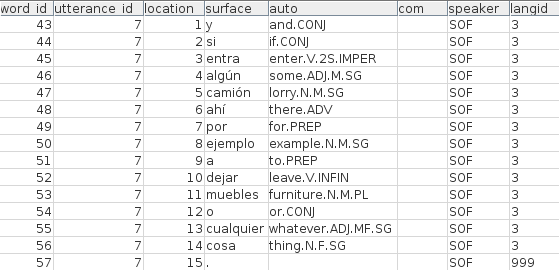
\includegraphics[width=\textwidth]{words_table.png}
  \end{figure}
  % Spanish sentence from the Miami corpus.
  % At this stage the autogloss field would be empty - that is what we're going to add now.
\end{frame}


\begin{frame}
\frametitle{\begin{small}\insertframenumber/\inserttotalframenumber\end{small} Lookup}
\begin{itemize}
\item Each word is looked up against the appropriate dictionary
\item Uses the language id assigned to the word
\item Writes out all ``hits'' in the CG input format
% 
\end{itemize}
\end{frame}


\begin{frame}
\frametitle{\begin{small}\insertframenumber/\inserttotalframenumber\end{small} Segmentation}
\begin{itemize}
\item Lookup also does some basic segmentation
\item Minimises number of dictionary entries \\ (\textbf{break} above)
\item Welsh: mutated words are tagged
% I better summarise what mutation is
    \begin{itemize}
    \item thad \textrightarrow tad (\textit{father}) + am
    \item gael \textrightarrow cael (\textit{get}) + am
    \end{itemize}
\item Spanish: clitic pronouns are tagged  
    \begin{itemize}
    \item ponerle \textrightarrow poner (\textit{put}) + le[pron.mf.3s]
    \item déjanos \textrightarrow dejar (\textit{leave})+ nos[pron.mf.1p]
    \end{itemize}
\end{itemize}
\end{frame}


\begin{frame}
\frametitle{\begin{small}\insertframenumber/\inserttotalframenumber\end{small} Mutation}
\begin{itemize}
\item \textbf{tad} (father)
    \begin{itemize}
    \item \textbf{ei \underline{d}ad} (\underline{his} father)
    \item \textbf{ei \underline{th}ad} (\underline{her} father) 
    \end{itemize}
\item \textbf{marw} (die, dead)
    \begin{itemize}
    \item \textbf{mae o'n \underline{m}arw} (he is dying)
    \item \textbf{mae o'n \underline{f}arw} (he is dead)
    \end{itemize}
\item direct object following a verb
    \begin{itemize}
    \item \textbf{Mi werthodd y ffermwr y \underline{m}ochyn}\\ (The farmer sold the pig)
    \item \textbf{Mi werthodd y ffermwr \underline{f}ochyn}\\ (The farmer sold a pig)
    \end{itemize}
\end{itemize}
\end{frame}


\begin{frame}[fragile]
\frametitle{\begin{small}\insertframenumber/\inserttotalframenumber\end{small} Welsh before CG}
\begin{footnotesize}
\begin{BVerbatim}
"<ddim>"
    "dim"  {96,1} [cy] n m sg :nothing: [208789] + sm
    "dim"  {96,1} [cy] adv :not: [204176] + sm
"<yn>"
    "yn"  {96,2} [cy] stat :stative: [200654]
    "yn"  {96,2} [cy] prep :in: [204430]
    "gan"  {96,2} [cy] prep :with: [196964] + sm
"<gynnar>"
    "cynnar"  {96,3} [cy] adj :early: [209212] + sm
"<iawn>"
    "iawn"  {96,4} [cy] adv :OK: [207540]
    "iawn"  {96,4} [cy] adv :very: [203775]
\end{BVerbatim}
\\ \hfill\textit{(Patagonia corpus, patagonia1)}
\end{footnotesize}
\\ ``\textit{not very early}''
\end{frame}


\begin{frame}[fragile]
\frametitle{\begin{small}\insertframenumber/\inserttotalframenumber\end{small} Welsh after CG}
\begin{footnotesize}
\begin{BVerbatim}
"<ddim>"
    "dim" {96,1} [cy] adv :not: [204176] + sm
"<yn>"
    "yn" {96,2} [cy] stat :stative: [200654]
"<gynnar>"
    "cynnar" {96,3} [cy] adj :early: [209212] + sm
"<iawn>"
    "iawn" {96,4} [cy] adv :very: [203775]
\end{BVerbatim}
\\ \hfill\textit{(Patagonia corpus, patagonia1)}
\end{footnotesize}
\\ ``\textit{not very early}''
\end{frame}
 

\begin{frame}[fragile]
\frametitle{\begin{small}\insertframenumber/\inserttotalframenumber\end{small} Spanish before CG}
\begin{footnotesize}
\begin{BVerbatim}
"<vamos>"
    "ir"  {122,3} [es] v 1p pres :go: [115789]
"<a>"
    "a"  {122,4} [es] prep :to: [1]
"<hacerle>"
    "hacer"  {122,5} [es] v infin :do: [62577] + le[pron.mf.3s]
"<el>"
    "el"  {122,6} [es] det.def m sg :the: [45129]
"<baño>"
    "baño"  {122,7} [es] n m sg :bathroom: [16011]
    "bañar"  {122,7} [es] v 1s pres :bathe: [16010]
\end{BVerbatim}
\\ \hfill\textit{(Patagonia corpus, patagonia1)}
\end{footnotesize}
\\ ``\textit{we're going to do the bathroom}''
\end{frame}


\begin{frame}[fragile]
\frametitle{\begin{small}\insertframenumber/\inserttotalframenumber\end{small} Spanish after CG}
\begin{footnotesize}
\begin{BVerbatim}
"<vamos>"
    "ir" {122,3} [es] v 1p pres :go: [115789]
"<a>"
    "a" {122,4} [es] prep :to: [1]
"<hacerle>"
    "hacer" {122,5} [es] v infin :do: [62577] + le[pron.mf.3s]
"<el>"
    "el" {122,6} [es] det.def m sg :the: [45129]
"<baño>"
    "baño" {122,7} [es] n m sg :bathroom: [16011]
\end{BVerbatim}
\\ \hfill\textit{(Miami corpus, sastre1)}
\end{footnotesize}
\\ ``\textit{we're going to do the bathroom}''
\end{frame}


\begin{frame}
\frametitle{\begin{small}\insertframenumber/\inserttotalframenumber\end{small} English Segmentation}
\begin{itemize}
\item Elisions are tagged
    \begin{itemize}
    \item gonna \textrightarrow go \# to.prep
    \item we're \textrightarrow we \# be.v.pres
    \end{itemize}
\item Plurals or verbs (3p sg pres) are tagged
    \begin{itemize}
    \item breaks \textrightarrow break \# pv
    \end{itemize}
\item Adjectives or verbs (past or pastpart) are tagged
    \begin{itemize}
    \item constructed \textrightarrow construct \# av
    \end{itemize}
\item Adjectives, singular nouns or verbs (prespart) are tagged
    \begin{itemize}
    \item thinking \textrightarrow think \# asv
    \end{itemize}
\end{itemize}
\end{frame}


\begin{frame}[fragile]
\frametitle{\begin{small}\insertframenumber/\inserttotalframenumber\end{small} English before CG}
\begin{footnotesize}
\begin{verbatim}
"<it's>"
    "it"  {545,1} [en] pron.sub 3s :it: [130342] # gb
"<coming>"
    "come"  {545,2} [en] sv infin :come: [82193] # asv
"<out>"
    "out"  {545,3} [en] adv :out: [157287]
"<on>"
    "on"  {545,4} [en] prep :on: [156077]
"<D_V_D>"
    "D_V_D"  {545,5} [en] name
"<then>"
    "then"  {545,6} [en] adv :then: [208154]
\end{verbatim}
\hfill\textit{(Miami corpus, herring7)}
\end{footnotesize}
\end{frame}


\begin{frame}[fragile]
\frametitle{\begin{small}\insertframenumber/\inserttotalframenumber\end{small} English after CG}
\begin{footnotesize}
\begin{verbatim}
"<it's>"
    "it" {545,1} [en] pron.sub 3s :it: [130342] # be.v.3s.pres
"<coming>"
    "come" {545,2} [en] v prespart :come: [82193] #
"<out>"
    "out" {545,3} [en] adv :out: [157287]
"<on>"
    "on" {545,4} [en] prep :on: [156077]
"<D_V_D>"
    "D_V_D" {545,5} [en] name
"<then>"
    "then" {545,6} [en] adv :then: [208154]
\end{verbatim}
\hfill\textit{(Miami corpus, herring7)}
\end{footnotesize}
\end{frame}


\begin{frame}
\frametitle{}
\begin{center}
\begin{huge} Multilingual disambiguation \end{huge}
\end{center}
\end{frame}


\begin{frame}
\frametitle{\begin{small}\insertframenumber/\inserttotalframenumber\end{small} Multiple languages}
\begin{itemize}
\item Ensure that each ``hit'' in the input file is tagged for language
\item Put all the rules into one grammar file, grouped according to language
\item Constrain the rules to act only on one language by including that language's tag in the rule
% I'll give some examples now
\end{itemize}
\end{frame}


\begin{frame}
\frametitle{\begin{small}\insertframenumber/\inserttotalframenumber\end{small} Sample rule}
\begin{itemize}
\item select (n) if (-1 (ord));
\item choose the noun reading if the preceding word is an ordinal
\item select ([es] n) if (-1 ([es] ord));
\item applies only to Spanish (\textbf{el primer viaje})
% 
\end{itemize}
\end{frame}


\begin{frame}[fragile]
\frametitle{\begin{small}\insertframenumber/\inserttotalframenumber\end{small} Welsh/Spanish}
\begin{footnotesize}
\begin{BVerbatim}
"<mewn>"
    "mewn" {128,4} [cy] prep :in:
"<motor>"
    "motor" {128,5} [es] n m sg :motor:
"<newydd>"
    "newydd" {128,6} [cy] adj :new:
"<internacional>"
    "internacional" {128,7} [es] adj m sg :international:
\end{BVerbatim}
\\ \hfill\textit{(Patagonia corpus, patagonia2)}
\end{footnotesize}
\\ ``\textit{in a new international motor-car}''
\end{frame}


\begin{frame}[fragile]
\frametitle{\begin{small}\insertframenumber/\inserttotalframenumber\end{small} Spanish/English}
\begin{footnotesize}
\begin{BVerbatim}
"<con>"
    "con" {60,1} [es] prep :with: [132994]
"<el>"
    "el" {60,2} [es] det.def m sg :the: [45129]
"<address>"
    "address" {60,3} [en] n sg :address: [55976]
"<de>"
    "de" {60,4} [es] prep :of: [33387]
"<aquí>"
    "aquí" {60,5} [es] adv :here: [11385]
\end{BVerbatim}
\\ \hfill\textit{(Miami corpus, zeledon5)}
\end{footnotesize}
\\ ``\textit{with the address from here}''
\end{frame}


\begin{frame}[fragile]
\frametitle{\begin{small}\insertframenumber/\inserttotalframenumber\end{small} Welsh/English}
\begin{footnotesize}
\begin{BVerbatim}
"<ac>"
    "ac" {27,1} [cy] conj :and: [209088]
"<oedd>"
    "bod" {27,2} [cy] v 3s imperf :be: [74724]
"<o>"
    "fo" {27,3} [cy] pron m 3s spoken :he: [209264]
"<gynno>"
    "gan" {27,4} [cy] prep+pron m 3s :with_him: [207424]
"<fo>"
    "fo" {27,5} [cy] pron m 3s :he: [196922]
"<background>"
    "background" {27,6} [en] n sg :background: [64983]
"<ddu>"
    "du" {27,7} [cy] adj :black: [209631] + sm
\end{BVerbatim}
\\ \hfill\textit{(Siarad corpus, deuchar1)}
\end{footnotesize}
\\ ``\textit{and it was \dots it had a black background}''
\end{frame}


\begin{frame}
\frametitle{\begin{small}\insertframenumber/\inserttotalframenumber\end{small} Cross-boundary rules}
\begin{itemize}
\item Rules can apply across language boundaries
\item Remove the language constraint when appropriate
% 
\end{itemize}
\end{frame}


\begin{frame}[fragile]
\frametitle{\begin{small}\insertframenumber/\inserttotalframenumber\end{small} Spanish adjective}
\begin{footnotesize}
\begin{BVerbatim}
"<es>"
    "ser"  {500,1} [es] v 23s pres :be: [51318]
"<otro>"
    "otro"  {500,2} [es] adj m sg :other: [83612]
    "otro"  {500,2} [es] pron m sg :other: [83613]
"<zip>"
    "zip"  {500,3} [en] n sg :zip: [1758]
"<code>"
    "code"  {500,4} [en] n sg :code: [81254]
\end{BVerbatim}
\\ \hfill\textit{(Miami corpus, sastre1)}
\end{footnotesize}
\\ ``\textit{it's another zipcode}''
\end{frame}


\begin{frame}
\frametitle{\begin{small}\insertframenumber/\inserttotalframenumber\end{small} Spanish adjective rule}
\begin{itemize}
\item \textbf{otro} can be an adjective before a noun, or a pronoun
\item The selection rule leaves the noun unspecified as to language:
\item select ([es] adj) if (1 (n));
\item \textit{adjective} will be selected before \textbf{any} \textit{noun} (not just Spanish)
% 
\end{itemize}
\end{frame}


\begin{frame}[fragile]
\frametitle{\begin{small}\insertframenumber/\inserttotalframenumber\end{small} Spanish adjective output}
\begin{footnotesize}
\begin{BVerbatim}
"<es>"
	"ser" {500,1} [es] v 23s pres :be: [51318]
"<otro>"
	"otro" {500,2} [es] adj m sg :other: [83612]
"<zip>"
	"zip" {500,3} [en] n sg :zip: [1758]
"<code>"
	"code" {500,4} [en] n sg :code: [81254]
\end{BVerbatim}
\\ \hfill\textit{(Miami corpus, sastre1)}
\end{footnotesize}
\\ ``\textit{it's another zipcode}''
\end{frame}


\begin{frame}[fragile]
\frametitle{\begin{small}\insertframenumber/\inserttotalframenumber\end{small} English verb}
\begin{footnotesize}
\begin{BVerbatim}
"<cada>"
    "cada"  {79,5} [es] adj mf sg :every: [18541]
"<vez>"
    "vez"  {79,6} [es] n f sg :time: [116758]
"<que>"
    "que"  {79,7} [es] conj :than: [93349]
    "que"  {79,7} [es] conj :that: [93350]
"<nos>"
    "yo"  {79,8} [es] pron.obl mf 1p :us: [80717]
"<vamos>"
    "ir"  {79,9} [es] v 1p pres :go: [115789]
"<camping>"
    "camp"  {79,10} [en] sv infin :camp: [74449] # asv
\end{BVerbatim}
\\ \hfill\textit{(Miami corpus, sastre1)}
\end{footnotesize}
\\ ``\textit{every time that we go camping}''
\end{frame}


\begin{frame}
\frametitle{\begin{small}\insertframenumber/\inserttotalframenumber\end{small} English verb rule}
\begin{itemize}
\item \textbf{camping} can be an adjective, a singular noun, or a verb
\item \textit{be thinking, enjoy reading, go fishing} 
\item In \textbf{vamos camping}, we can get the correct end tag by specifying the meaning of the preceding verb, rather than the lemma:
\item substitute (sv infin asv) (v prespart) \\([en] sv infin asv) (-1 ([en] "be") or (:go:) );
\item The tags on \textbf{camping} are rewritten to tag it as a present participle 
% 
\end{itemize}
\end{frame}


\begin{frame}[fragile]
\frametitle{\begin{small}\insertframenumber/\inserttotalframenumber\end{small} English verb output}
\begin{footnotesize}
\begin{BVerbatim}
"<cada>"
    "cada" {79,5} [es] adj mf sg :every: [18541]
"<vez>"
    "vez" {79,6} [es] n f sg :time: [116758]
"<que>"
    "que" {79,7} [es] pron.rel :that: [93350]
"<nos>"
    "yo" {79,8} [es] pron.obl mf 1p :us: [80717]
"<vamos>"
    "ir" {79,9} [es] v 1p pres :go: [115789]
"<camping>"
    "camp" {79,10} [en] v prespart :camp: [74449] #
\end{BVerbatim}
\\ \hfill\textit{(Miami corpus, sastre1)}
\end{footnotesize}
\\ ``\textit{every time that we go camping}''
\end{frame}


\begin{frame}
\frametitle{}
\begin{center}
\begin{huge} Rule types and \\language type \end{huge}
\end{center}
\end{frame}


\begin{frame}
\frametitle{\begin{small}\insertframenumber/\inserttotalframenumber\end{small} Removal}
\begin{itemize}
\item ``Delete'' items from the dictionary
\item Homonym selection
\item select ("cyfeiriad" [cy] :direction:);
\item Archaic/infrequent words
\item remove ("tasu" [cy] :stack:);
% 
\end{itemize}
\end{frame}


\begin{frame}
\frametitle{\begin{small}\insertframenumber/\inserttotalframenumber\end{small} Compensate}
\begin{itemize}
\item Remove words which are an artefact of the lookup
\item remove ([cy] "mynd" v 2s imper nm);
\item \textit{nos} $<$ \textit{dos}
\item remove ([in] "gum" n sg sm);
\item \textit{um} $<$ \textit{gum}
% 
\end{itemize}
\end{frame}


\begin{frame}
\frametitle{\begin{small}\insertframenumber/\inserttotalframenumber\end{small} English}
\begin{itemize}
\item substitute (n sg pv) (n pl) ([en] n sg pv);
\item \textit{house} \textrightarrow \textit{houses}
\item substitute (as) (adj) ([en] as) (1 ([en] n) or ([en] pron));
\item \textit{a miniature rabbit, miniature ones}
% 
\end{itemize}
\end{frame}

\begin{frame}
\frametitle{\begin{small}\insertframenumber/\inserttotalframenumber\end{small} English}
\begin{itemize}
\item substitute (pron.sub) (pron.obj) ([en] pron.sub) (-1 ([en] v infin));
\item \textit{and open it}
\item substitute (sv infin av) (v past) ([en] sv infin av) (-2 ([en] pron.sub)) (-1 preverbal);
\item \textit{they closed}
% 
\end{itemize}
\end{frame}


\begin{frame}
\frametitle{\begin{small}\insertframenumber/\inserttotalframenumber\end{small} English}
\begin{itemize}
\item substitute (av past) (v past) ([en] av past) (-1 ([en] pron.sub)) (not -1 (have.v.pres)) (not -2 ("have"));
\item \textit{we bought}, \textbf{not} \textit{you've done, we have bought}
\item substitute (av past) (v pastpart) ([en] av past) (-1 (have.v.pres) or ("have") or ("be") or (det.def) or (det.indef));
\item \textit{you've done, you have done, it was misspent, un rebuilt}
% 
\end{itemize}
\end{frame}


\begin{frame}
\frametitle{\begin{small}\insertframenumber/\inserttotalframenumber\end{small} English}
\begin{itemize}
\item Refine existing tags
\item substitute (123p) (1p) ([en] v 123p) (-1 (pron.sub 1p));
\item \textit{we are}
\item In general, more dependent on rule order
% 
\end{itemize}
\end{frame}


\begin{frame}
\frametitle{\begin{small}\insertframenumber/\inserttotalframenumber\end{small} Default choices}
\begin{itemize}
\item When left with an [or], we can make a ``default`` choice
\item select ([cy] v infin) if (0C ([cy] v infin) or ([cy] v 3s imper));
\item \textit{cerdded}
\item C enforces the two conditions
% 
\end{itemize}
\end{frame}


\begin{frame}
\frametitle{\begin{small}\insertframenumber/\inserttotalframenumber\end{small} Careful \dots}
\begin{itemize}
\item Scope of \textbf{remove} can be unexpected
\item Likewise \textbf{select-if-not}
\item select (imper) if (not @1 ("ni"));
\item Caused 304 regressions in Spanish output!
% 
\end{itemize}
\end{frame}


\begin{frame}
\frametitle{\begin{small}\insertframenumber/\inserttotalframenumber\end{small} Rule numbers}
\begin{itemize}
\item Spanish: 150 
\item Welsh: 180
\item English: 200
% 
\end{itemize}
\end{frame}


\begin{frame}
\frametitle{\begin{small}\insertframenumber/\inserttotalframenumber\end{small} Output method}
\begin{itemize}
\item CG writes out the disambiguated text
\item This file is parsed
\item The glosses (lexeme + POS tag) are inserted into the words table
\item The words are then written out to create the autoglossed file
% 
\end{itemize}
\end{frame}


\begin{frame}
\frametitle{\begin{small}\insertframenumber/\inserttotalframenumber\end{small} The words table}
  \begin{figure}[h]
  \centering
  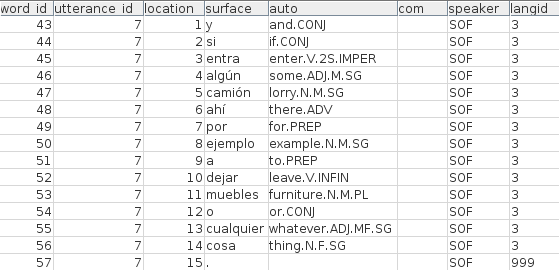
\includegraphics[width=\textwidth]{words_table.png}
  \end{figure}
  % Spanish sentence from the Miami corpus.
  % The autogloss field is now filled.
\end{frame}


\begin{frame}
\frametitle{}
\begin{center}
\begin{huge} Accuracy \end{huge}
\end{center}
\end{frame}


\begin{frame}
\frametitle{\begin{small}\insertframenumber/\inserttotalframenumber\end{small} Accuracy}
\begin{center}
\begin{tabular}{ccccc}
& \begin{small}\textit{Words}\end{small} & \begin{small}\textit{Coverage}\end{small} & \begin{small}\textit{MFL}\end{small} & \begin{small}\textit{Accuracy}\end{small} \\
\cline{1-5}\noalign{\smallskip}
\textbf{Welsh-Spanish} & 15,677 & 100\% & W:92\% & 99\% \\
(Patagonia\footnote{patagonia1,2,3,6}) & & & \\
\textbf{Spanish-English} & 4,202 & 97\% & S:59\% & 97\% \\
(Miami\footnote{zeledon5}) & & & \\
\textbf{Welsh-English} & 10,411 & 96\% & W:81\% & 98\% \\
(Siarad\footnote{stammers4, deuchar1}) & & & \\
\end{tabular}
\end{center}
\end{frame}


\begin{frame}
\frametitle{\begin{small}\insertframenumber/\inserttotalframenumber\end{small} Dictionary coverage}
\begin{center}
\begin{tabular}{cccc}
& \begin{small}\textit{Words}\end{small} & \begin{small}\textit{Nouns}\end{small} & \begin{small}\textit{}\end{small} \\
\cline{1-4}\noalign{\smallskip}
\textbf{Welsh} & 209k & 6k & 3\% \\
\textbf{Spanish} & 130k & 19k & 15\% \\
\end{tabular}
\end{center}
\end{frame}


\begin{frame}
\frametitle{\begin{small}\insertframenumber/\inserttotalframenumber\end{small} Speed}
\begin{itemize}
\item 900-1100 words per minute
\item 1 minute to autogloss 5 minutes of manually-glossed speech
\item Siarad: 500,000 words in 8h27m
% 
\end{itemize}
\end{frame}


\begin{frame}
\frametitle{\begin{small}\insertframenumber/\inserttotalframenumber\end{small} Sample utterances}
\begin{footnotesize}

\textbf{*SER:}   dw@1 i@1 (y)n@1 hopeless@2 efo@1 tynnu@1 llun@1 . \%snd:"deuchar1"\_72848\_73881

\textit{\%gls:}   be.1S.PRES PRON.1S PRT hopeless with take.NONFIN picture

\textit{\%eng:}   I'm hopeless at drawing

\textbf{*MYF:}   +$<$ \&=laugh . \%snd:"deuchar1"\_73196\_73881

\textbf{*SER:}   dw@1 i@1 (y)n@1 tynnu@1 llun@1 i@1 [/] i@1 (y)r@1 plant@1 $<$i@1 plant@1$>$ [//] $<$i@1 (y)r@1$>$ [//] \# i@1 er@0 \&h Helen@0 a@1 Susanna@0 a@1 +/. \%snd:"deuchar1"\_73881\_79477

\textit{\%gls:}   be.1S.PRES PRON.1S PRT take.NONFIN picture for for DET children for children for DET for IM Helen and Susanna and

\textit{\%eng:}   I draw a picture for \dots for the children, for, er, Helen and Susanna and \dots

\end{footnotesize}
\begin{small}
\hfill\textit{(Siarad corpus, deuchar1)}
\end{small}
% Hesitation markers, delivery hints, elision
\end{frame}


\begin{frame}
\frametitle{\begin{small}\insertframenumber/\inserttotalframenumber\end{small} Typesetting}
  \begin{figure}[h]
  \centering
  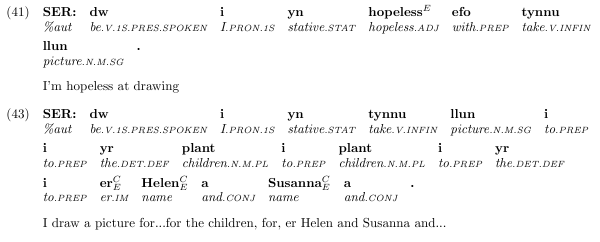
\includegraphics[width=\textwidth]{deuchar1.png}
  \end{figure}
  % Spanish sentence from the Miami corpus.
  % At this stage the autogloss field would be empty - that is what we're going to add now.
\end{frame}


\section{Adding value}

\subsection{Texts}

\begin{frame}
\frametitle{\begin{small}\insertframenumber/\inserttotalframenumber\end{small} Texts}
\begin{itemize}
\item Check on typos -- proof-reading
% several % typo rate - these lead to misalignment in the autoglosser, but they also cause problems for MOR
\item Consistent glosses
% meddwl not ``consider'' in one place, and ``think'' in another
\item More granular analysis
\item Global tag changes or enrichment
\end{itemize}
\end{frame}


\subsection{Data-mining}

\begin{frame}
\frametitle{\begin{small}\insertframenumber/\inserttotalframenumber\end{small} Data-mining}
\begin{itemize}
\item Interactive webpages (\textit{bangortalk.org.uk})
\item Easier or more detailed statistical analysis with R
\item Input to machine translation. speech-to-text, etc
\end{itemize}
\end{frame}


\begin{frame}
\frametitle{}
\begin{center}
\begin{huge} thinkopen.org.uk/git \end{huge}
\end{center}
\end{frame}


\end{document}